\documentclass{article}

\usepackage{comment}
\usepackage{graphicx}
\graphicspath{ {./} }
\usepackage{corl_2022} % Use this for the initial submission.
%\usepackage[final]{corl_2022} % Uncomment for the camera-ready ``final'' version.
%\usepackage[preprint]{corl_2022} % Uncomment for pre-prints (e.g., arxiv); This is like ``final'', but will remove the CORL footnote.

\title{An Off-Policy Approach to Learning in the Game of Pokemon}

% The \author macro works with any number of authors. There are two
% commands used to separate the names and addresses of multiple
% authors: \And and \AND.
%
% Using \And between authors leaves it to LaTeX to determine where to
% break the lines. Using \AND forces a line break at that point. So,
% if LaTeX puts 3 of 4 authors names on the first line, and the last
% on the second line, try using \AND instead of \And before the third
% author name.

% NOTE: authors will be visible only in the camera-ready and preprint versions (i.e., when using the option 'final' or 'preprint'). 
% 	For the initial submission the authors will be anonymized.

\author{
  Steven Callahan\\
  Department of Computer Science\\
  University of Texas at Austin
  United States\\
  \texttt{stevencallahan@utexas.edu} \\
  %% examples of more authors
  %% \And
  %% Coauthor \\
  %% Affiliation \\
  %% Address \\
  %% \texttt{email} \\
  %% \AND
  %% Coauthor \\
  %% Affiliation \\
  %% Address \\
  %% \texttt{email} \\
  %% \And
  %% Coauthor \\
  %% Affiliation \\
  %% Address \\
  %% \texttt{email} \\
  %% \And
  %% Coauthor \\
  %% Affiliation \\
  %% Address \\
  %% \texttt{email} \\
}


\begin{document}
\maketitle

%===============================================================================

\begin{abstract}
    The game of Pokemon is suprisingly complex and difficult to model. As such, applications of reinforcement learning on the game have seen limited success due to inaccuracies in simulators and the relative ineffectiveness of common reinforcement learning methods. Certain approaches have also not been feasible due to the inability for certain approaches to overcome the adversary they train against, particularly when trained against high-performing opponents. This paper attempts to solve this issue by making taking a bi-directional, off-policy approach to contextual bandits and thus be agnostic of the behavior policy's performance.
\end{abstract}

% Two or three meaningful keywords should be added here
\keywords{Pokemon, Learning} 

%===============================================================================

\section{Introduction}
	
\quad	Pokemon is the largest grossing media franchise in the world~\citep{Wikipedia}, with a variety of mediums in which it is present. The Pokemon series of video games feature a turn-based combat system that is easy to learn, but incredibly hard to master.

\quad	In this battle system, generally speaking, players each have up to six pokemon each and (in a competitive setting) can choose for their active pokemon to either use one of four moves, or to switch into one of their benched pokemon. Moves can do damage, inflict status effects, change stats of yourself or the enemy, or even change variables about the battlefield itself, like the weather or the force of gravity.

\quad	Given the complexity of the game, there are very few accurate simulations of Pokemon battles, and even fewer that are open-source, thus limiting the ability to apply reinforcement learning methods to the game.

\quad	Given all of these variables, attempts at applying traditional RL techniques to a Pokemon battle are incredibly varied. Here, I make two contributions to this field:

\quad	1. An integration of reinforcement learning with the command-line Pokemon Battle Simulator in the Pokemon Showdown! Github Repository~\citep{Showdown}.

\quad	2. An opponent-agnostic approach to learning.

%===============================================================================

\section{Related Work}
\label{sec:related_work}

\quad	Previous work in the field has seen varied success, due in large part to the creation or use of a greatly simplified simulator that cannot be applied to a "real" Pokemon battle~\citep{CalebLewis}~\citep{Akshay}. Thus, a goal in this project is an attempt at integrating a reinforcement learning framework with a reliable and accurate Pokemon battle simulator, as used in~\citet{KevinChen}, called "Pokemon Showdown". Showdown is an open-source fan recreation of the game's battle engine that is used for competitive play, so its accuracy is among the highest of any simulator.

\quad Another interesting issue raised in~\citet{KevinChen} is that on-policy methods fail to converge to an optimal policy against high-level opponents due to their inability to find positive rewards. Such is the inspiration for "bi-directional" learning in this paper, where an agent can still learn positive rewards in the training phase, even if it's losing.

\quad While the majority of reinforcement learning techniques applied to Pokemon are derivative of Q-learning~\citep{CalebLewis}~\citep{Akshay}~\citep{KevinChen}~\citep{RodrigoRill}, applications beyond this have been attempted as well, such as Policy Gradient~\citep{JosephFlaherty} and Neural Network Classification~\citep{RodrigoRill2}, with limited success and applicability to the goals of this paper. Applications of Policy Gradient~\citep{Sutton} and Apprenticeship Learning~\citep{Pieter}~\citep{MyProf}, were considered, but due to time and resource constraints simpler methods were instead applied. 

%===============================================================================

\section{Pokemon Battles}
\label{sec:battles}

\quad	This section will cover the peculiarites of Pokemon battles as a game to apply reinforcement learning to, as well as why certain decisions were made in this particular paper. Due to the complexity and intricacies of pokemon battles, prerequisite knowledge of Pokemon is important. Those unfamiliar with the battle system can get a brief overview \href{https://bulbapedia.bulbagarden.net/wiki/Pokemon_battle}{here}.

\quad	We will be making some simplifications to the game of Pokemon here to make reinforcement learning more applicable. Namely, we will be assuming a "competitive" setting for a pokemon battle. This means items cannot be used and difficulty-reducing features like the ability to switch pokemon following a player knockout are not enabled. Furthermore, we can assume all pokemon present are reasonably powerful such that every pokemon present has some amount of competitive viability.

\quad	We will further assume the following to further simplify our model:

\quad	- We'll be only considering battles in the first generation of Pokemon. This means newer additions to the series, like EVs, Pokemon Abilities, Held Items, Weather Effects, and other complex moves do not need to be considered.

\quad - The AI will not be trained on switching Pokemon; it will use moves with the currently active Pokemon until it is knocked out. When this happens, a new Pokemon is chosen randomly.

\quad	- Teams are randomly generated using the Pokemon Showdown random team generator. This is used because team selection is a large part of human competitive pokemon, which this paper does not attempt to address. Random battling has its own competitive scene which lends itself much better to an AI.

\quad	The first peculiarity is the Pokemon themselves; while in a game like chess pieces can only move in a particular pattern (with a few exceptions) such as rooks always moving cardinally and bishops diagonally; in a Pokemon battle each Pokemon can know up to four of a large number of moves. These moves cannot be changed in the middle of battle, but this means a Pikachu in one battle may not have the same moves as a Pikachu in another battle.

\quad	An interesting approach could be to model an enemy's potential moves as a distribution of moves this pokemon has used in training with moves the enemy uses then being "confirmed" for that battle. However, this approach has two major caveats:

\quad	- It is heavily reliant on training data representative of real-world application, which has its own caveats when considering an off-policy approach to learning.

\quad	- In a competitve setting, most Pokemon aren't present on the field long enough to use all of their moves, so it's most likely that a distribution of an enemy Pokemon's moves will be the main reliance. Therefore, one can simply ignore enemy move choice altogether since the move the enemy will use is for all intents and purposes stochastic, and thus can be taken into account just by that Pokemon being on the field.

\quad	Another peculiarity of Pokemon battles is the order in which "turns" are executed; both players choose moves simultaneously, with the turn order then being chosen by a complex series of "priorities". Generally speaking, however, switching Pokemon will occur before moves are executed, and the pokemon with the higher speed stat will move first. If a Pokemon is knocked out between the time a command is issued and it's able to use the move, the knocked out Pokemon will not use its move and the turn is essentially wasted.

\quad	We can avoid mis-attributions of no reward to a move because it didn't get executed for some reason by only counting a move as "used" when the Pokemon actually gets to use the move, rather than issuing the command to use a particular move.

\quad	A third peculiarity is that moves don't always have a clear nor immediate effect. For example, the move "Mirror Move" will use the move the enemy previously used. Other status-changing moves are difficult to quantify, since their effects may only be seen many turns later, if at all.

\quad	The approach taken in this paper doesn't have a good way of integrating this information into state-action-value tuples, and thus addressing this issue will be left to future works.

%===============================================================================

\section{Agents}
\label{sec:agents}

\quad	Two types of agents are used in this paper, with each using slightly different information for the state:

\quad	- SingleAgent uses the enemy pokemon and the move being used as the state.

\quad	- DoubleAgent uses the player's pokemon, the enemy pokemon, and the move being used as the state.

\quad	The inclusion of the player's active pokemon in the state has a few notable implications. Firstly, the "Same Type Attack Bonus" or STAB, which increases the power of a move by 50\% if the user is the same type as the move, would be apparent based on the state. This would not be captured in SingleAgent. Furthermore, DoubleAgent's value estimates would be more finely tuned to the situation at hand, whereas SingleAgent's would be a composite of any pokemon with a particular move against a given enemy pokemon.

\quad	The drawback to including the player's pokemon in the state space is, of course, that the state space grows much larger than before. Specifically, it grows by a factor of $n$, where $n$ is the number of possible pokemon. Applying this to our simplified generation 1 state space, the state space will expand from 24,915 to 3,762,165~\citep{PokemonWiki}.

\quad	The goal in setting up the states in this way between the two agents is to measure the tradeoff between expanding the state space and its effect on coverage, performance, and training time:

\quad\quad	- coverage is the percentage of states at testing time that have been visited at least once during training. If a state has not been seen yet, the model will default to giving that state a value of zero.

\quad\quad	- performace is the agent's ability to win battles, which is distinct from the reward function (described below). Performance is measured as a percentage of battles won.

\quad\quad	- training time is how long it takes for the agent to train. Comparing the two agents with the same number of iterations of training may not be fair because DoubleAgent may take longer to train up to the same number of iterations, so we can instead cut off training time at a particular threshold to make performance estimates more fair.

\quad	The reward function is the decimal difference between the enemy's HP before and after the turn ends, with an additional reward of one given and taken for a knockout against your opponent and yourself respectively. This is modeled as zero-sum; the reward for one player is equal to the negative reward of the other.

\quad	Rewards are taken at the end of a battle, so learning will occur all at once between iterations. Values for each state are stored as the average reward gained for each time that situation was visited.

\quad Due to the simplified state space and issues with integrating the simulator, we precompute all pokemon-move pairs before the battle begins and reference them as a table throughout the battle; a total of 36 matchups are possible in a 6v6 space, so computationally this operation is relatively cheap.

\quad	As mentioned in the introduction, a bi-directional approach to learning is taken. That is, while the agent is only controlling one side of the battlefield, they can see the actions and outcomes of the opponent and learn from them as well. There are two motivations for this decision:

\quad\quad - The agent will learn twice as fast because it evaluates two states per turn of battle as opposed to one.

\quad\quad - There is potential for the agent to "learn" from a smarter opponent by observing the states they visit.

%===============================================================================

\section{Experiments}
\label{sec:experiment}

\quad	There are three questions I aim to answer/reinforce:

\quad\quad - Is including the active pokemon in the state space worth the expansion of the state space?

\quad\quad - Can an agent train better against a smarter opponent? Furthermore, can the student become the master?

\quad\quad - What kind of playstyle does the given reward function lend itself to? Does it work "properly"?

\quad In all experiments, a "Training" and "Testing" phase are undergone:

\quad\quad - In the training phase, 1,000 iterations of battles are undergone. In each iteration, teams are randomly generated, followed by five battles with the teams. Five battles are run to help remove variability in the reward estimates (e.g. moves can miss or critically hit, multiplying the reward by a factor of 0 or up to 2 respectively). This means each agent will train on a total of 5,000 battles of 1,000 unique 6v6 scenarios. Agents train in an off-policy manner; namely, they choose random moves to ensure every state-action pair is reachable given enough iterations of battle, regardless of the opponent being trained against. The time taken to complete the iterations is also measured.

\quad\quad - Once the agent is trained, 1,000 iterations of testing are done. In each iteration, teams are randomly generated, followed by a single battle, where the results are tallied and output.

\quad As mentioned earlier, there are a few different testing metrics used:

\quad\quad - Performance: The winrate of the agent against a specified opponent. This will usually be against a random opponent, though for certain tests we will evaluate performance against another trained agent.

\quad\quad - Training Time: How long it took for the training to execute.

\quad\quad - Coverage: The amount of states visited in testing that were also visited in training. This measures the applicability of learned information; it doesn't matter how good training was if it only applies to a small fraction of the space encountered in testing.

\quad\quad To get a better understanding of the time-performance tradeoff between the SingleAgent and the DoubleAgent, we will train two different versions of DoubleAgent: a "Matched" agent that trains for as long as the SingleAgent takes, and a "Full" agent that gets to train for the full 5,000 battles. 

\quad To measure the ability of an agent to "learn" from a smarter opponent, we train a fresh SingleAgent, referred to as SingleStudent, against the previously trained SingleAgent, now referred to as SingleMaster, for 5,000 iterations. Testing is then performed against the SingleMaster for the same 1,000 battles. 

\quad Finally, we will do a brief analysis on the commonly used moves by the Agents and build a high-level description of the Agents from their preferences.

%===============================================================================

\section{Experimental Results}
\label{sec:result}
	
\quad EXPERIMENT 1: TRADEOFFS IN EXPANDING THE STATE SPACE

\quad	Below are training times for a SingleAgent and DoubleAgent.

	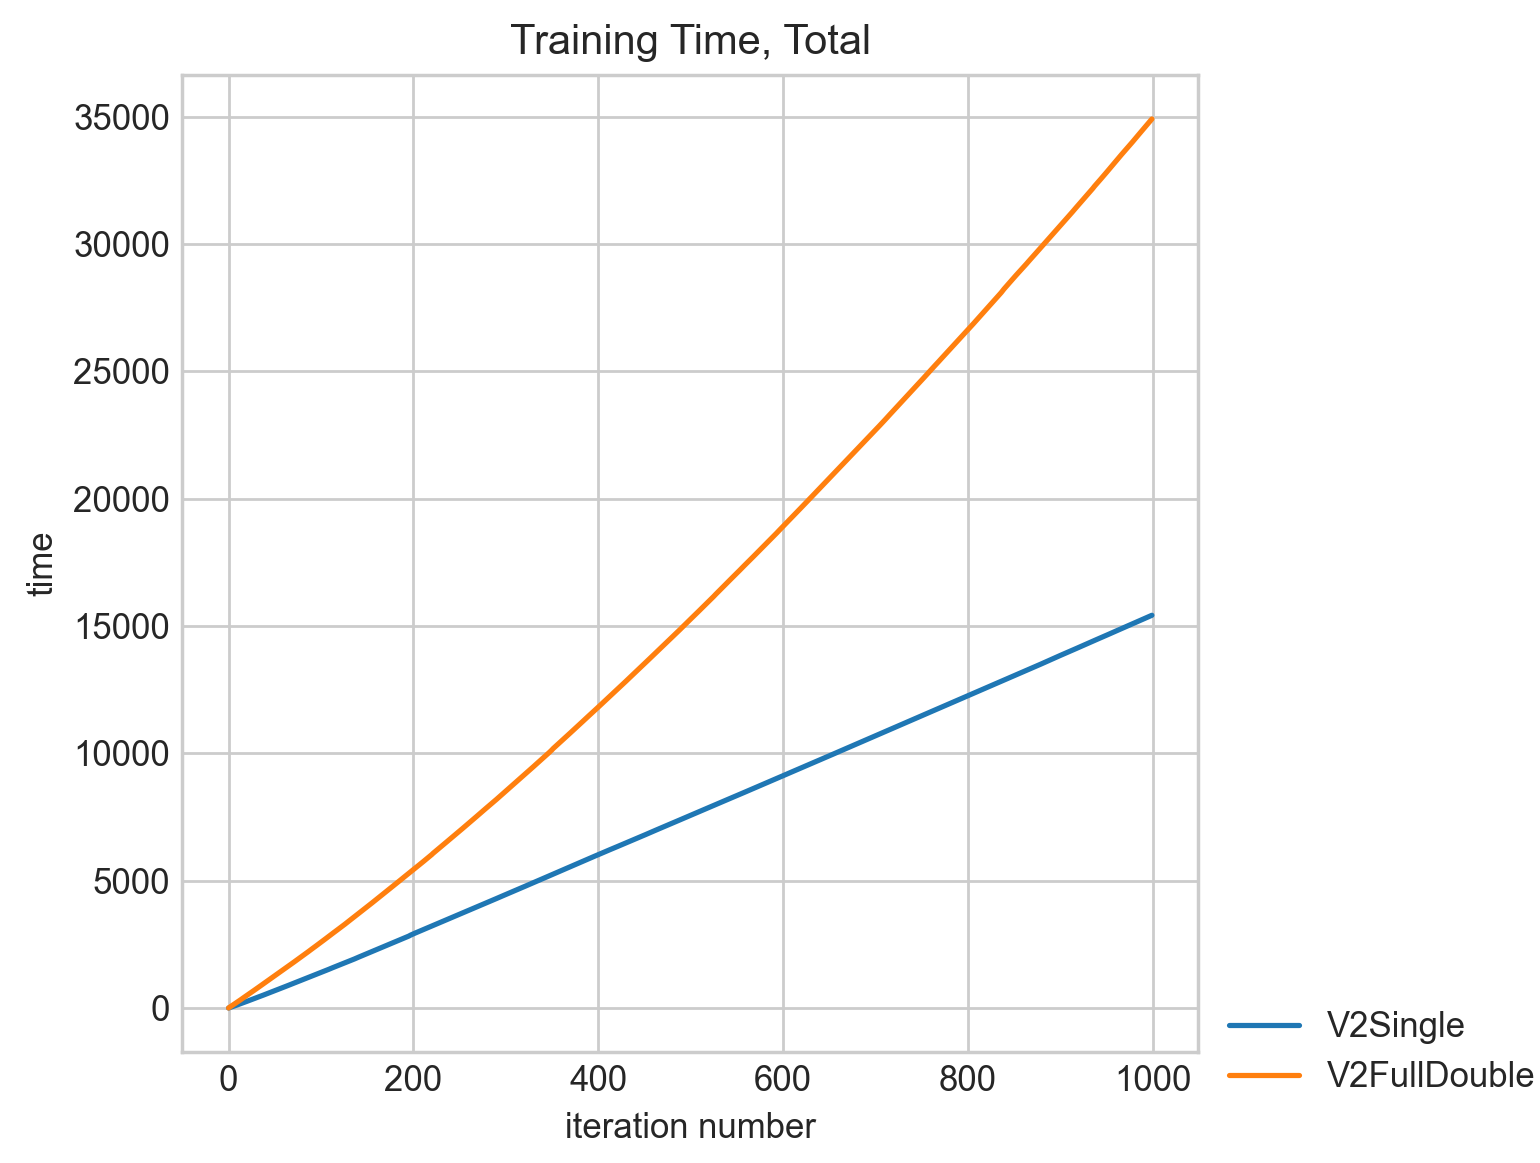
\includegraphics[scale=.3]{Total Training Time}

\quad	Figure 1: The training time required to train a SingleAgent and DoubleAgent to completion.

\quad As expected, the DoubleAgent requires significantly more time to train, as it is managing a larger table of state-action values.

\quad The MatchedDoubleAgent was able to train through 646 iterations (3237 battles) before exceeding the time it took for SingleAgent to finish 1,000, which based on the training curves shown in Figure 1 should actually be around 500. I am not completely sure as to why the times are different, though it could be due to variability in computation speed of my laptop.

	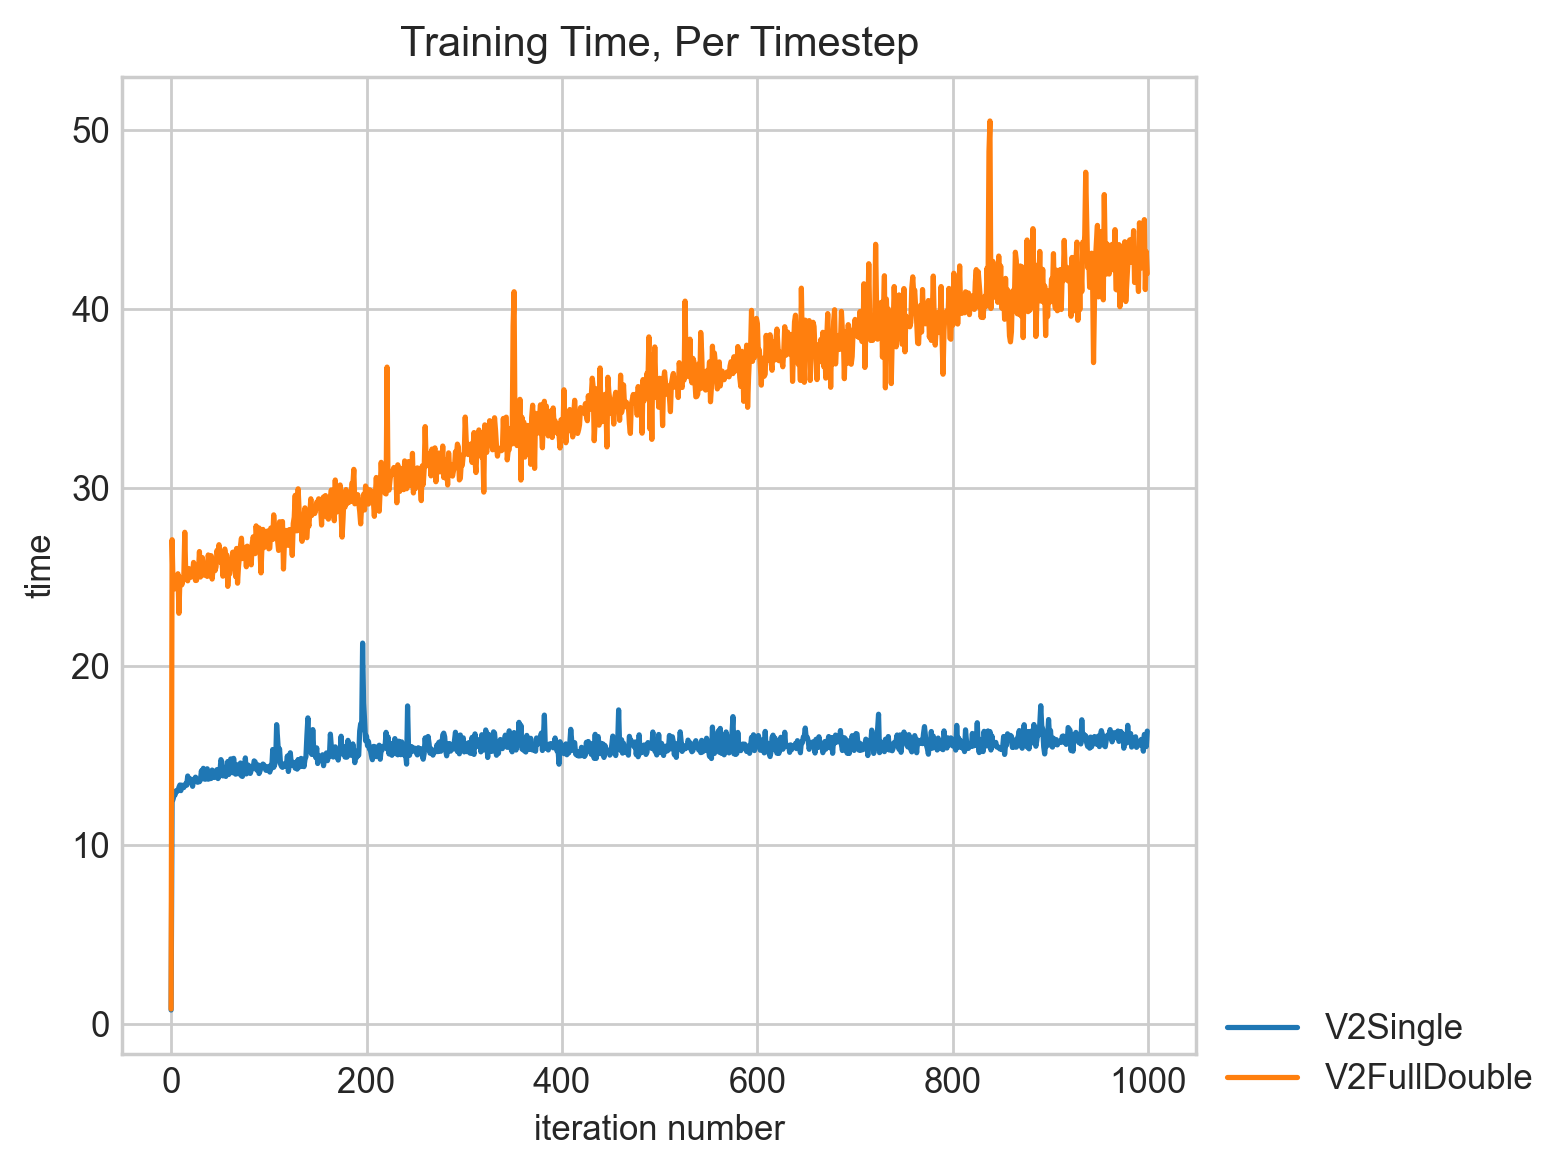
\includegraphics[scale=.3]{Per-Timestep Training Time}

\quad	Figure 2: The per-timesstep training time required to train a SingleAgent and DoubleAgent to completion.

\quad Interestingly, the SingleAgent seems to converge in its per-timestep training time after roughly 300 iterations, whereas the DoubleAgent's time increases linearly and does not converge in the 1,000 iterations. This is an indicator that 5,000 random battles is insufficient for convergence for the DoubleAgent, which we will explore more below.

\quad	The trends seen in these time results are similar for other variations on the Single and Double agents, so to avoid redundancy we won't re-state them.

\quad After training, the winrate of the agents against a randomly acting adversary is as follows:

	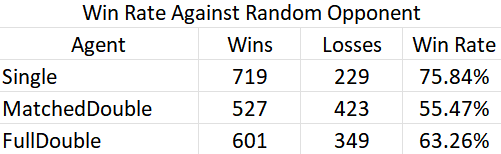
\includegraphics[scale=1]{Win Rate}

\quad Figure 3: The winrates of the SingleAgent, MatchedDoubleAgent, and FullDoubleAgent.

\quad Suprisingly, the SingleAgent displays a strong advantage against both MatchedDoubleAgent and FullDoubleAgent, despite the former training for the same amount of time and the latter training for the same number of iterations. This is likely due to neither agent converging to an optimal policy, which is supported by the coverage tables below:

	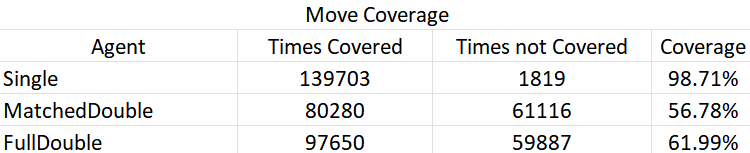
\includegraphics[scale=.7]{Coverage}

\quad Figure 4: The coverage of the agents. Recall that a "covered" state is a state seen during testing which had also been seen during training.

\quad We see for both the MatchedDouble and FullDouble agents that their coverage is relatively low compared to SingleAgent, which likely explains their poor performance against the random adversary- often times they're performing random moves as well. Furthermore, given the improvements to the coverage and win rate of the FullDoubleAgent relative to the MatchedDoubleAgent, it is very likely training the FullDoubleAgent for more iterations will improve performance further.

\quad EXPERIMENT 2: LEARNING FROM SMARTER OPPONENTS

\quad Below is the performance of the SingleStudent against the SingleMaster:

	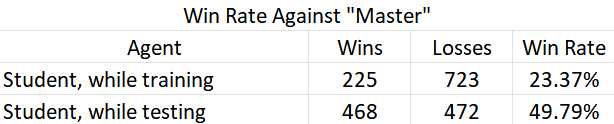
\includegraphics[scale=1]{StudentMasterWinRate}

\quad Figure 5: The winrate of the SingleStudent.

\quad During training the student is making random actions, so the winrate is consistent with the above SingleAgent's winrate as seen in Figure 3. Interestingly, the Student performs exactly as well as the Master, meaning either the hypothesis about learning from a smarter opponent is incorrect or that in both cases the SingleAgent converged to an optimal policy given the limited state space. It is likely that the Student converges to said optimal policy faster than the SingleAgent did due to seeing the "best" actions to take from the SingleMaster, although this cannot be verified as-is. Due to time constraints I was unable to verify this through experiementation, though as mentioned in the conclusion this is a ripe topic of future work.

\quad As seen above, due to the inability for the DoubleAgent to converge to an optimal policy, the lack of convergence conflicts with the hypothesis we want to test- if a "student" can learn from a "master" it battles against- since even the FullDoubleAgent is not really a "master". Furthermore, the performance against the theoretical DoubleMaster (or lack thereof) could not be attributed to the hypothesis since the lack of convergence itself is a cause for poor performance. For this reason DoubleStudent and DoubleMaster tests have been omitted.

\quad EXPERIMENT 3: ANALYSIS OF MOVE PREFERENCES

\quad The top five moves the SingleAgent prefers are:

\quad\quad Hyper Beam, with a value of .505

\quad\quad High Jump Kick, with a value of .459

\quad\quad Earthquake, with a value of .401

\quad\quad Hydro Pump, with a value of .400

\quad\quad Psychic, with a value of .399

\quad These are all incredibly strong damage-dealing moves, which we hypothesized the reward function would lend itself to. Interestingly, the top two moves are both glitched in their Generation 1 appearances to make them more powerful:

\quad\quad - Hyper Beam usually takes two turns to execute (one turn is a cooldown turn to balance out the high damage the move deals), but this effect would not occur if the opposing pokemon was knocked out, which was fairly likely due to the high damage of the move.

\quad\quad - High Jump Kick was intended to deal severe recoil damage if it misses, but this recoil was only a flat 1 HP in Generation 1. For reference, virtually all competitively viable Pokemon have hundreds of HP, so this recoil is negligible.

\quad It's interesting that the SingleAgent was able to identify these moves as favorable; although it didn't recognize them as "glitched", it did recognize their potency, which many human players wouldn't be able to do since the underlying effects of the move being glitched aren't apparent.

\quad We also hypothesized status moves would be heavily penalized, which they did turn out to be. Below are the highest ranking moves that don't deal damage:

\quad\quad Substitute, with a value of -.022

\quad\quad Rest, with a value of -.045

\quad\quad Softboiled, with a value of -.056

\quad\quad Recover, with a value of -.076

\quad\quad Barrier, with a value of -.088

\quad Substitute is likely the top entry because it creates a "decoy" that the enemy has to break before being able to damage the opponent, meaning if the agent uses it first they will be immune to damage for the rest of the turn.

\quad Rest, Softboiled, and Recover all heal the user by a fraction of their max HP; Rest is a full heal (which also puts you to sleep for two turns; the agent cannot detect this since it doesn't consider status conditions), whereas Recover and Softboiled are up to 50\%. However, since the agent is training randomly, it's likely the HP gained is far lower than that value, if any at all (it's possible the move is being used at full HP, in which case no HP will be restored). Including the player's current HP would likely help the agent determine when it's best to use these "recovery" moves.

\quad Barrier is a support move that doubles the user's defense, meaning they'll take half damage from physical attacks. Since most powerful attacks are physical (the top three entries the AI prefers all deal physical damage), it's likely the lack of damage taken in that turn is recognized in the value function, despite no possibility for damage to occur as a result of it.

\quad Thus, while the SingleAgent wasn't able to prefer support moves over damage-dealing moves, it was able to determine which support moves are useful relative to each other. However, given that the policy is deterministic, it is unlikely for a support move to perform well if chosen repeatedly. Therefore, future work that aims to elicit non-damage moves from an AI needs to be stochastic.

\quad Suprisingly, the results for the DoubleAgent are more or less identical to that of the SingleAgent. From this we can draw two conclusions:

\quad\quad - The DoubleAgent is correctly learning which moves are best (at least relative to the SingleAgent), so its lack of performance lies in its inability to generalize this information over the state space. This is further supported by the lack of coverage.

\quad\quad - There is an "optimal policy" relative to the DoubleAgent that we simply haven't reached in 5,000 battles.

%===============================================================================

\section{Conclusion \& Future Work}
\label{sec:conclusion}

\quad The SingleAgent was able to converge to a respectable 75\% win rate against a random adversary and an impressive 98\% coverage of situations in testing. While the DoubleAgents did not perform as well in the same amount of training time, it is very likely they could perform better if either a way to generalize across the data was created or further training was executed.

\quad Using the opposing Pokemon 's performance yielded mixed results, and ultimately more work will need to be done on this "student-master"/bi-directional approach to verify or reject it. Specifically, doing an analysis on the SingleStudent's performance as it approaches convergence and measuring the iterations it takes to match the performance of the SingleMaster would verify or refute this hypothesis.

\quad The damage-dealing moves the agents prefer to use correlate well with competitive consensus of moves in that category, and while the agents were unable to prefer status moves over said damage-dealing moves, they were still able to adequately determine which status moves were useful relative to other status moves.

\quad A disadvantage to the approach taken here is that the agent's decision-making is not stochastic, meaning it will always use a certain move in a given state. That being said, the agent also lends itself to using effective damage-dealing moves, meaning it won't be in the same state for very long, and using damage-dealing moves does lend itself well to winning against low-elo opponents (i.e. random actors). In any case, to emulate good competitive play, a stochastic policy should be trained instead of a deterministic one. This is surely an area of future work.

\quad Other areas to expand upon include expanding the state space, finding ways to generalize the state space to an increased number of states, and applications of more intricate Reinforcement Learning methods, like Policy Gradient.

\quad Additionally, although the integrated simulator works in this configuration, it is quite fragile and difficult to expand to future work due to the Pokemon-Showdown framework being written in typescript, whereas most reinforcement learning libraries are in Python, meaning a great deal of cross-language communication is necessary. This is especially true for any functions that require computation during battle, such as any stochastic action. For this reason, future work should include a rewriting of the battle-running functionality to better support these functions.

%===============================================================================

% The maximum paper length is 8 pages excluding references and acknowledgements, and 10 pages including references and acknowledgements

\clearpage
% The acknowledgments are automatically included only in the final and preprint versions of the paper.
\acknowledgments{If a paper is accepted, the final camera-ready version will (and probably should) include acknowledgments. All acknowledgments go at the end of the paper, including thanks to reviewers who gave useful comments, to colleagues who contributed to the ideas, and to funding agencies and corporate sponsors that provided financial support.}

%===============================================================================

% no \bibliographystyle is required, since the corl style is automatically used.
\bibliography{StevenCallahanFinalProject}  % .bib
\begin{comment}
@misc{,
  author       = {}, 
  title        = {},
  howpublished = {},
  month        = ,
  year         = ,
  note         = {Accessed: --2022}
}
\end{comment}
\end{document}
